\startonecol \chapter[Gaussian tricks]{Hypothesis testing with the CLT} \label{gauss} \endonecol

This chapter covers most of what we traditionally learn in first-year statistics. 
\comment{
Much of it is obsolete. It covers parameters which we know to have a Normal (aka Gaussian) distribution,
or those things which are derived therefrom. These are nice because the math has already been done, by
people who lived before computers, meaning that we don't need metaphorically heavy machinery to do most of
the calculations here.} Most of the work will consist of taking a dot product, maybe inverting a matrix,
and then looking up a number in a table. 

Everything here depends on the Central Limit Theorem, and more
generally, assumes that your real-world data has a textbook
distribution. Typically, the textbooks state that as the number of draws
$n \to \infty$, the distribution is correct, but whether it is correct
for your data set is a question of \ind{asymptotic theory}.

If your data doesn't fit the CLT, one option is to work out how your
data is distributed, 
and then write down a likelihood function. If you are
looking to estimate model parameters, do a maximum likelihood estimation;
if you are looking to test a hypothesis, write down a likelihood ratio
based on the distribution you have just calculated.
Another alternative is to use the Monte Carlo methods of 
Chapter \ref{boot} to determine the properties of your model for $n$ 
significantly smaller than infinity.


\section{Models and constraints} A \vocab{hypothesis} is a constraint
on otherwise unconstrained parameters. 

For example, given four variables named $Y$, $X_1$, $X_2$, and $X_3$,
one could estimate the $\beta$s in the equation
\begin{equation*}
Y = \beta_0 + \beta_1 X_1 + \beta_2 X_2 + \beta_3 X_3 + \epsilon
\end{equation*}
using a standard OLS regression as per the last chapter.

Frequently, the parameters and the model happen to match very closely.
For example, if we believe that $Y$ is an affine linear sum of $X_1$,
$X_2$, $X_3$, then we are making a claim that 
\begin{equation*}
Y = \alpha_0 + \alpha_1 X_1 + \alpha_2 X_2 + \alpha_3 X_3.
\end{equation*}
Given the parameters estimated using OLS, translating those parameters
to the model is rather trivial:
\begin{align*}
\alpha_0 &= \beta_0\\
\alpha_1 &= \beta_1\\
\alpha_2 &= \beta_2\\
\alpha_3 &= \beta_3.
\end{align*}
However, one may have a model where the translation between parameter estimates and model
parameters is a little more complex.
For example, let us say that we are measuring bicycle usage in a city
($B$).
It would be a function of the number of motorists $M$, the city's
population $P$, the physical size of the city $S$,  and measures of
the availability of public transportation $T$. But we know that the
availability of public transportation is also a function of the city's
population and physical size. Thus, our model is
\begin{align*}
B &= \alpha_0 M + \alpha_1 P + \alpha_2 \sqrt{S} + \alpha_3 T\\
T &= \alpha_4 P + \alpha_5 \sqrt{S}.
\end{align*}

One option for estimating this model is to run two analogous regressions,
\begin{align*}
B &= \beta_0 M + \beta_1 P + \beta_2 \sqrt{S} + \beta_3 T + \epsilon\\
T &= \beta_4 P + \beta_5 \sqrt{S} + \epsilon.
\end{align*}
Now the correspondence between the two parameters is as trivial as
before ($\alpha_0=\beta_0$, $\alpha_1=\beta_1$, et cetera). This is the
simplest example of \vocab{exactly solved parameters}.
But we get a
distorted view of the effect of city size and population on bicycling
prevalence, because some of those variables' effect is subsumed in the fact that
those factors help to determine whether a city has public
transportation. If the population of a city rises ten percent, ridership
will not rise by $.1 \beta_1$, because $T$ will change as well.

Another option is to substitute $T$ as specified in the second equation into
the first. Then, the model is
\begin{align*}
B &= \alpha_0 M + (\alpha_1 +\alpha_3 \alpha_4) P + (\alpha_2 + \alpha_3 \alpha_5) \sqrt{S}.\\
\end{align*}
The OLS analogue of a linear equation still looks like it did before:
\begin{align*}
B &= \beta_0 M + \beta_1 P + \beta_2 \sqrt{S} + \epsilon.
\end{align*}
Now, the conversion is nontrivial:
\begin{align}
\alpha_0 &= \beta_0     \label{consteq1}\\
\alpha_1 +\alpha_3 \alpha_4 &= \beta_1        \label{consteq2}\\
\alpha_2 + \alpha_3 \alpha_5 &= \beta_2.       \label{consteq3}
\end{align}
Equation \ref{consteq1} still gives us an estimate of $\alpha_0$,
but all our information about  $\alpha_1$ through $\alpha_5$ is
embodied in Equations \ref{consteq2} and \ref{consteq3}. With four
unknowns and two equations, the parameters are \airq{oversolved}. 
\index{undersolved parameter}

We have a better view of the effect of the variable $P$ on $B$, but we
do not have enough information to disaggregate that effect into the
direct effect ($\alpha_1$) and the indirect effect ($\alpha_3 \alpha_4$)
caused by the effect population has on public transport availability
($\alpha_4$). 

Depending on your situation and goals, one setup or the other may be
more appropriate. However, we must acknowledge the limitations of an
undersolved system: $n$ parameter estimates can inform at most $n$ model
parameters.

Now, let us say that a prior study has shown that $\alpha_2= 2.204$.
Discarding the equation for $T$ for now, our model is now:
\begin{align*}
B &= \alpha_0 M + \alpha_1 P + \alpha_2 \sqrt{S} + \alpha_3 T\\
\alpha_2 &= 2.204.
\end{align*}
and after estimating the parameters using a simple OLS estimation, the 
translation from estimated $\beta$s to model $\alpha$s is:
\begin{align*}
\alpha_0 &= \beta_0\\
\alpha_1 &= \beta_1\\
\alpha_2 &= \beta_2\\
\alpha_2 &= 2.204\\
\alpha_3 &= \beta_3.
\end{align*}
Unless we have the incredible luck that $\beta_2=2.20400$, $\alpha_2$ is an
\vocab{oversolved parameter} that has no solution.

There are two things that one can do with an oversolved system. One is
to use the extra constraints to inform the parameter estimation routine;
in the example above, we would estimate the parameters under the
assumption that $\beta_2$ is fixed at 2.204.
You can do this using constrained least squares (Section
\ref{constrainedls}) or via maximum likelihood estimation as in Chapter
\ref{mle}. The other option is to compare the unconstrained version of
the model with the constrained version to see how much distortion occurs
when the constraint binds. This is \airq{testing the constraints}, aka,
a \airq{hypothesis test}.
\index{least squares!constrained}

Recall that the two primary activities of the statistician are
estimating models and testing models. 
For an undersolved system, we can neither estimate 
nor test the model. For an exactly solved system, we can always
estimate the parameters of the model, but can not verify or refute the
model: you give me a data set, and I will always be able to give you some set of model
parameters. For an oversolved system, we can both estimate the parameters
and test whether the model is correct, because there will not always
be a way to consistently transform the estimated parameters into model
parameters.

Because there is so little persuasive power in an estimated but not
tested model, we often make up
ways to convert an exactly solved system into an oversolved one.
For example, one could add to any equation the additional equation
$\alpha_i = 0$ for all $i$.
By specifying
$Y = \alpha_0 + \alpha_1 X_1 + \alpha_2 X_2 + \cdots$ and $\alpha_1=0$,
we have an oversolved system whose validity we can test. Indeed, this
is the system of equations behind the $t$-tests that are universally
reported with every regression.

This may seem like belaboring the language with such a simple system,
but it is easy to extend this framework to systems of equations, 
exotic constraints, and other variants of the mapping from parameter
estimates to model parameters and testing oversolved equations.

By the way, a statement like `We reject
the claim $\alpha_1=0$' is only half right. We are actually rejecting
the claim that both
$Y = \alpha_0 + \alpha_1 X_1 + \alpha_2 X_2 + \cdots$ {\em and}
$\alpha_1=0$. 
The first and second equations are mathematically of equal
status, but the custom is to presume that only the second equation is a
subordinate equation which is under scrutiny. Thus, one would correctly
say `we reject this system of equations'. Having given this caveat, the
remainder of this chapter will use the traditional terminology that
takes the base model as given, reducing
the above pair of equations to the hypothesis $H_0: \alpha_1=0$.

The remainder of this chapter goes over the process of testing 
an oversolved system. The key to constructing a test is in knowing 
how the distribution of the data informs the likely distribution of
our estimates of the $\alpha$s, and the key to that process is the
Central Limit Theorem. The first part of this chapter will thus return
to probability theory, describing how the CLT affects various parameter
distributions, and then the remainder of the chapter considers how 
those parameter distributions can be used to test hypothesized models.

\section{Meet the Gaussian family} \label{dist2}
With the exception of the Normal, the distributions below are distinct
from the distributions of Section \ref{distlist}. The distributions
there
are typically used to describe data that we have observed in the real
world. But having gathered data, we often model the data using techniques
such as linear regressions, that produce means of model parameters,
model variances, and other parameters. Those model parameters have their
own distributions, and those are typically one of the distributions below.


\paragraph{The \ind{Central Limit Theorem}} The CLT is the first piece of magic
that we need. It tells us that:
$$\overline X \xrightarrow{a} \left[\mu,{\sigma^2\over n}\right].$$
In fact, we not only have $\overline X$ in the limit, but its distribution:
As $n\to \infty$, $$\sqrt{n} \frac{\left(\overline X - \mu\right)}{\sigma} \sim {\cal N}(0,1),$$ 
regardless of where $X$ came from. With that regularity of nature,
we can derive all of the following distributions.  \label{CLT}

\subsection{Normal\index{Normal distribution}} 

The Normal distribution, defined on page \pageref{normal},
will also be used to describe some of the parameters derived below.
The big problem with the Normal distribution is that it depends on $\sigma$, an
unknown. It also depends on $\mu$, but if the statistic
being tested is unbiased---like most of the estimators of $\beta$ in the
catalog from Chapter \ref{projections}---then you have $\mu$. Thus, much of the trickery in the
section on test design below involves combining distributions in ways
such that the unknown $\sigma$s cancel out.

\begin{itemize}
\item $\{{\cal N} (a,b)\} + \{{\cal N} (c,d)\} \sim {\cal N}
(a+c,b+d)$ (where $\{x\}$ indicates a variable with the given distribution).
\end{itemize}

\subsection{$\chi^2$ distribution}\index{chi squared distribution@$\chi^2$ distribution} $[\sum_n (x-\overline
x)^2]/\sigma^2\sim \chi^2_{n-1}$. The numerator there is the sample
variance times $n$, so we can test that the sample variance equals a
given $\sigma^2$ with this. But unless we assume $\sigma$ like that,
we are up the same creek as with the Normal.

\begin{itemize}
\item $\{{\cal N} (0,1)\}^2 \sim \chi^2_1$

\item $\{\chi^2_1\}$ + \dots + ($n$ of these) + \dots + $\{\chi^2_1\} \sim \chi^2_n$

\end{itemize}			\label{chisq}

Notice that the sample variance is $\sim
\chi^2_{n-1}$, not $n$, because given the first $n-1$ data points, the
last one can actually be calculated from that data; meaning that we
effectively have the sum of $n-1$ $\{\chi^2_1\}$s plus a no longer
stochastic constant.

\subsection{Student's t distribution\index{t distribution}} Let $\uv$ be
a vector of data (such as the error terms in a regression). Then
${\overline X - \mu \over S/\sqrt{n}}\sim
t_{n-1}$, where $S=\uv'\uv/n$ (a scalar). This is a work of genius by
Mr. Student.\footnote{\airq{Mr. Student} is actually Mr. William Sealy
Gosset, who published the t test in 1908 based on his work as an employee
of the Guiness Brewery. \index{Student} \index{William S Gosset}}
By dividing a normal by $\sqrt{\chi^2_{n-1}\over (n-1)}$, the unknown
$\sigma$s cancel, and we have a function whose elements are all known,
and its distribution.  If $n=2$, we call it a Cauchy distribution.
\label{tstat}


\subsection{$F$ distribution\index{F distribution}}  This is the same cancel-the-$\sigma$s trick as with the $t$, but here the form
is $[\chi^2_m/m]/[\chi^2_n/n]\sim F(m,n)$. For example, if the numerator
is a ${\cal N}(0,1)$, and the denominator is a $\chi^2$ based on the
sample variance, then this is the square of the $t$ statistic.
The nice thing about the $t$ distribution is that it is easy and it
allows one-tailed hypothesis tests. But if you want to test a
multivalued hypothesis, then you need to do an $F$ test.

\subsection{Lookup tables}
There are three things that cover most of what you will be doing with a
distribution: finding values of its PDF, values of its CDF, and inverse
values of its CDF.
Here are the functions to look up the value of the PDF at a given point:

\begin{lstlisting}
double gsl_ran_gaussian_pdf (double X, double SIGMA);
double gsl_ran_tdist_pdf (double X, double NU);
double gsl_ran_fdist_pdf (double X, double NU1, double NU2);
double gsl_ran_chisq_pdf (double X, double NU);
\end{lstlisting}

The prefix \cinline{gsl\_ran} indicates that these
functions are from the random number generation module
(\cinline{gsl/gsl\_randist.h}. Random number generation itself will be
delayed to page \pageref{randomnumbers}. Notice that there is no mean
for the Normal, so we may need to modify $X$ accordingly, e.g., if $X$
is drawn from a ${\cal N}(7,1)$, then you will need to ask the GSL for 
\cinline{gsl\_ran\_gaussian\_pdf(X-7, 1)}.


The next distribution calculation found in tables in the back of
statistics texts is calculating the CDF above or below a point. 
The \cinline{P-}functions below calculate the CDF below a point, i.e.
$\int_{-\infty}^X f(y) dy,$
while the \cinline{Q-}functions calculate the CDF above a point, i.e.
$\int^{\infty}_X f(y) dy.$
These will obviously add to one, so you can express any area in terms of whichever function is clearest.

For example, if we find that our Normally distributed mean is 2.2 standard
deviations above zero, then we can reject the one-tailed hypothesis that
the mean is zero with probability \cinline{1 - gsl\_cdf\_gaussian\_Q(2.2, 1) ==
gsl\_cdf\_gaussian\_P(2.2, 1)}.

Here is the list of functions:
\index{Gaussian distribution|see{Normal distribution}}
\index{chi squared distribution@$\chi^2$ distribution!gsl\_cdf\_chisq\_P@\cinline{gsl\_cdf\_chisq\_P}}
\index{t distribution!gsl\_cdf\_tdist\_P@\cinline{gsl\_cdf\_tdist\_P}}
\index{F distribution!gsl\_cdf\_fdist\_P@\cinline{gsl\_cdf\_fdist\_P}}
\index{Normal distribution!gsl\_cdf\_gaussian\_P@\cinline{gsl\_cdf\_gaussian\_P}}
\ttindex{gsl\_cdf\_...}
\begin{lstlisting}
double gsl_cdf_gaussian_P (double X, double SIGMA);
double gsl_cdf_tdist_P (double X, double NU);
double gsl_cdf_fdist_P (double X, double NU1, double NU2);
double gsl_cdf_chisq_P (double X, double NU);
\end{lstlisting}
\dots plus all of these with the \cinline{P} replaced by a \cinline{Q}.


In the other direction, we may want to know where we will need to be to reject a hypothesis with 95\%
certainty. For example, a value-at-risk oriented regulator will want to know what a bank is likely to lose 
one day in the month. That is, what is the value of the 1-in-20, or 5\%, point on the CDF?
Assuming a Normal(M,S) distribution of profit and loss,\footnote{This assumption is false. Securities
typically have \ind{leptokurtic} (fat-tailed) returns.} the bank will report a \ind{value at risk} of {\tt
gsl\_cdf\_gaussian\_Pinv (0.05, S)+M}. Here are the requisite function declarations:
\index{chi squared distribution@$\chi^2$ distribution!gsl\_cdf\_chisq\_Pinv@\cinline{gsl\_cdf\_chisq\_Pinv}}
\index{t distribution!gsl\_cdf\_tdist\_Pinv@\cinline{gsl\_cdf\_tdist\_Pinv}}
\begin{lstlisting}
double gsl_cdf_gaussian_Pinv (double X, double SIGMA);
double gsl_cdf_chisq_Pinv (double P, double NU);
double gsl_cdf_tdist_Pinv (double P, double NU);
\end{lstlisting}
\dots plus all of these with the \cinline{P}s replaced by \cinline{Q}s.
Notice that there is no inverse for the CDFs of the F distribution.





\section{Testing a hypothesis}




We have all the ingredients we need to test a hypothesis; all that
remains is to glue them all together. For example, in the last chapter, the code
found the coefficient vector \cinline{beta} and \cinline{xpx\_inv}, which is the
variance-covariance matrix of \cinline{beta}.  Now assume that \cinline{beta}
is normally distributed (for example, the original data set consists
of iid draws from a homoskedatic distribution). Then we can use the
above functions to find the probability that each element of \cinline{beta}
is different from zero:

\lstset{texcl=true}
\begin{lstlisting}
//We enter with the vector $\betav$ and matrix {\tt xpx\_inv}
int i;
double confidence[beta->size];
for (i=0;i< beta->size; i++){
    confidence[i] = gsl_cdf_gaussian_Q(abs(gsl_vector_get(beta,i)), gsl_matrix_get(xpx_inv, i,i));
    confidence[i] -= .5;
    confidence[i] *= 2;
}
\end{lstlisting}
\lstset{texcl=false}
The last two steps converted from the one-tailed area below \cinline{beta}
to a two-tailed area between $\pm$\cinline{beta}.


\subsection{The t-test} \label{ttest} \index{t test|(textbf}
\index{t test!apop\_t\_test@\cinline{apop\_t\_test}}
\index{t test!apop\_paired\_t\_test@\cinline{apop\_paired\_t\_test}}
Among the most common and simplest questions one asks is: are two 
sets of observations from the same process? Chapter \ref{sql} already showed how one
would do such a test; let us briefly revisit the process now.
Let \cinline{n\_side} be the income of households
drawn from the side of town North of the railroad tracks, and
\cinline{s\_side} be the income of households drawn from the South side of
town. Are North side incomes different from South side incomes? 

If $\mu$,
$\sigma^2$, and $n$ are the estimated mean, variance, and actual count
of elements of each data set,
$${\mu_a + \mu_b \over \sqrt{\sigma^2_a/n_a + \sigma^2_b/n_b}} \sim t_{n_a + n_b -2}.$$
Using the ingredients above, the reader could construct a function to
test the hypothesis that the number above, the $t$-statistic, is
different from zero for any given confidence level. Apophenia provides a
high-level function to do the work for you:

\cindex{apop\_t\_test}
\begin{lstlisting}
gsl_vector *a = gather_data("n_side");
gsl_vector *b = gather_data("s_side");
apop_data  *t = apop_t_test(a, b);
apop_data_show(t);
\end{lstlisting}
As per the discussion on page \pageref{testoutput}, Apophenia's testing
functions return a data table listing test statistics, degrees of
freedom, confidence, et cetera. You can print the entire set as above or
just pull a single element, e.g.,
\cindex{apop\_data\_get\_tn}
\begin{lstlisting}
double pval = apop_data_get_tn(t, "p_val%", 0);
\end{lstlisting}

Now let us say that the data is paired, in the sense that for each
element in the first set, there is an element in the second set that is
related; put another way, this means that for each element $a_i$, there
is a corresponding element $b_i$ such that the difference $a_i - b_i$
makes real-world sense. For example, we could look at student scores on
a test before a set of lessons and the same students after the lessons.
Then, rather than looking at the $t$-distribution for the before data
and comparing it to the $t$-distribution for the after data, we could
look at the vector of differences $a_i - b_i$ and test where zero falls
in the appropriate $t$-distribution. This is generally a more powerful test,
meaning that we are more likely to reject the null hypothesis of no
difference between the two vectors, therefore the paired $t$-test is
generally preferable over the unpaired version above (when it is
applicable). Apophenia provides the \cind{apop\_paired\_t\_test}
function to run this test where appropriate.
 \index{t test|)textbf}

\subsection{The $\chi^2$ test}
\index{chi squared test@$\chi^2$ test}

By itself, this is only useful for testing whether the sample variance
is equal to a given $\sigma^2$, because unless you assume $\sigma^2$ 
or are doing a homework question that says \airq{$\sigma^2$
is known}, you don't have it. Otherwise, in the case of multiple variables, you need to use
an $F$ test; see below.

$H_0$ asks, is ${\Qv'
\betav} = \cv$?  This is a very versatile question. E.g., $\Qv =
\vector{1\cr 0\cr 0}$ plus $\cv = [7]$ gives $H_0: \beta_1 = 7$. Or, $\Qv = \vector{1 \cr
-1}$ and $\cv = \vector{0}$ gives $H_0: \beta_1=\beta_2$. 
Or, say we want to test that $\beta_2 = 2\beta_3$. Then let $\Qv=\vector{0 \cr 1 \cr -2}$ and $\cv = 0$.
To test multiple hypotheses at once, simply stack the above:
\begin{equation}
\begin{matrix}\Qv' = \vector{1 & 0 & 0  \cr
                0 &1 &-2} 
                & \cv = \vector{7 \cr 0}\end{matrix}.\label{qc}\end{equation}

I dare
say that every linear hypothesis having to do with a mean or a $\beta$ can be
fit into this form.\footnote{If our concern is a mean, then set
$\Yv=$your data, $\Xv=$ a column of ones, and $\beta$ will then be
$\mu$. Recall that we typically expect that the first column of $\Xv$ to
be a column of ones anyway.}
Define $q$ to be the number of constraints (columns
of $\Qv$), $N$ the sample size, and $K$ the number of parameters to be
estimated ($\betav$).

Now, if $H_0$ is true and we are using OLS, then $\Qv' \betav \sim {\cal
N}(\cv, \sigma^2 \Qv' (\Xv'\Xv)^{-1} \Qv)$,\footnote{For any other
method, the variance is $\Qv'$(the variance from section
\ref{cat})$\Qv$.} and we can use all of the above. The $\chi^2$
statistic now becomes:

\begin{equation}		\label{chi1}
{(\Qv'\hat\betav - \cv)' [\Qv' (\Xv'\Xv)^{-1} \Qv]^{-1} (\Qv' \hat\betav - \cv)
\over \sigma^2} \sim \chi^2_q
\end{equation}

If we are testing a variance, we'd have 

\begin{equation}		\label{chi2}
{{\bf u}' {\bf u} \over \sigma^2} \sim \chi^2_{N-K}
\end{equation}


\subsection{The $F$ test\index{F test}}\label{ftestsec}

As above, we can divide Equation \ref{chi1} by Equation \ref{chi2}
to give us a statistic with an $F$ distribution and no unknown
$\sigma^2$ element:


\startonecol
\wideeqnbox{12cm}{
%\begin{equation}	
{N-K\over q}
{(\Qv'\hat\betav - \cv)' [\Qv' (\Xv'\Xv)^{-1} \Qv]^{-1} (\Qv' \hat\betav - \cv)
\over \uv' \uv } \sim F_{q,N-K}. \label{ftest}
%\end{equation}	
}
\endonecol

If you have read this far, you know how to code all of the operations
in Equation \ref{ftest}.  But fortunately, 
Apophenia includes a function that will calculate Equation \ref{ftest}
for you.
\index{F test!apop\_F\_test@\cinline{apop\_F\_test}}
To do this, you will need to feed the function a $\betav$ vector, and a
matrix $\Qv'$ plus a vector $\cv$ that indicate the set of hypotheses
you wish to test. Notice that each {\em row} of the input matrix represents a
hypothesis. Also, recall that functions ending in \cinline{calloc} allocate
a matrix or vector and simultaneously set every element to zero, giving
you a blank slate to fill. Thus, if you already have a data set, and
would like to run an OLS regression and then test the joint hypothesis
of Equation \ref{qc}, here's what you'd type:
\begin{lstlisting}
apop_estimate *e = apop_OLS.estimate(data, NULL);
gsl_matrix *Q   = gsl_matrix_calloc(3,2);
gsl_vector *c   = gsl_vector_calloc(2);
gsl_matrix_set(Q, 0, 0, 1);
gsl_matrix_set(Q, 1, 1, 1);
gsl_matrix_set(Q, 1, 2, -2);
gsl_vector_set(Q, 0, 7);
apop_F_test(e, data, Q, c);
\end{lstlisting}

Included in the default output from a regression,
many stats packages run an $F$-test that reports the
joint hypothesis that all coefficients are different from zero. That is,
it runs the $F$-test where $\Qv = {\bf I}$ and $\cv = {\bf 0}$.\footnote{This is
partly because this $F$-test can be calculated using only the $R^2$.
Once again, statistical convention is dictated by 70s computing power.
\index{R squared@$R^2$}}
It is up to you
to decide whether this is a relevant statistic for the situation you are
dealing with, but because it is a custom to report it, some
people expect it, so Apophenia facilitates this hypothesis test by
assuming it as the default when you send in {\tt NULL} variables:
\cinline{apop\_F\_test(estimate, data, NULL, NULL)}. That is,
if $\Qv'=$\cinline{NULL}, Apophenia assumes ${\bf Q}=={\bf I}$ and if
$\cv=$\cinline{NULL}, Apophenia assumes ${\bf c} == {\bf 0}$.




\comment{
\subsection{The F-test}
But we have the whole variance-covariance matrix to work with, not just
the diagonal, so we can readily test any joint hypothesis that suits
our fancy. First, we need a means of expressing the hypothesis.
}

\comment{
\section{Good ol' OLS}
This section would discuss how to write your very own \cinline{regress}
function, which, as noted above, just consists of solving for the $\beta$
in $(X'X)\beta = X'Y$.  The last chapter showed us the code to find the
betas with the smallest squared error; this section will cover testing
hypotheses about those betas.

\subsection{GLS} Generalized least squares refers to any method that
uses a variance-covariance matrix that isn't the identity matrix. Having
written our \cinline{regress} function, it's almost trivial to generalize
to GLS. But the fun of GSL is in working out what that matrix should be.
This section would give examples of favorites such as AR-1 processes
from time series analysis (and hey, why not AR-$N$?).

The easiest thing to do is simply calculate the variances and covariances of the data itself:

%\begin{verbatim}
\begin{lstlisting}
#include "gsl_convenience_fns.h"
gsl_vector_view one_col, another_col;
gsl_matrix *var_covar=gsl_matrix_alloc(data->size2, data->size2);
int i,j;

for(i=0;i< data->size2; i++){
   for(j=0;j<= i; j++){
      one_col = gsl_matrix_column(data, i);
      another_col = gsl_matrix_column(data, j);
      covar = cov(&one_col.vector, &another_col.vector);
      gsl_matrix_set(var_covar, i, j, covar);
      if (j!=i) gsl_matrix_set(var_covar, j, i, covar);
   }
}
\end{lstlisting}
%\end{verbatim}

Now that we've got this variance-covariance matrix, $\Sigma$, we can
apply the formula $\beta_{GLS} = (X'\Sigma X)^{-1} (X'\Sigma Y)$.
}

\comment{
This gives us  $N\cdot (N+1)/2$ covariances that need to be calculated; your data is probably not up to
the task of providing enough information to allow this to be estimated, in which case you will need to
compromise and impose some number of restrictions. 

For example, FGLS (Feasible GLS) assumes that the var-covar matrix is of the form 
$$\left[\matrix{
1 &\rho & \rho^2 & \rho^3\cr
\rho &1 & \rho  & \rho^2\cr
\rho^2 & \rho & 1 & \rho\cr
\rho^3 & \rho^2  & \rho &1\cr
}\right].$$
This makes life easy because we now only have one variable to estimate.
}

\section{Testing the assumptions} Errors have to be normally distributed, or else
the whole OLS system here does not apply. Many stats package user's manuals
suggest plotting the errors and then squinting at the picture; you can
do this using \cinline{apop\_plot\_histogram}. An
alternative is to use the higher moments of the distribution.
A Normal distribution has only two parameters,  the mean and the
standard deviation, and everything else about the Normal distribution is
defined therefrom. Notably, the third moment is zero, and the fourth
moment is $3 \sigma^4$. 
Un-normalized kurtosis $>3$ is known as \vocab{leptokurtic} and $<3$ is
known as \vocab{platykurtic}; see Figure \ref{tailfig} for a mnemonic.

\marginalia{Kurtosis minus three}{
There is some debate as to whether the kurtosis of a ${\cal N}(0,1)\equiv 3$
or $\equiv 0$. This is simply a definitional issue: some prefer to
normalize all reported kurtoses by subtracting three from the actual
fourth moment. For example, the GSL does the normalization; Apophenia does not.
Bear this in mind when interpreting kurtosis output. If you see a
negative kurtosis, then you are guaranteed that you are getting
normalized kurtosis, since a fourth power can never be negative.
\index{kurtosis}}

\begin{figure*}[tb]
\hspace{-.3in}\scalebox{0.7}{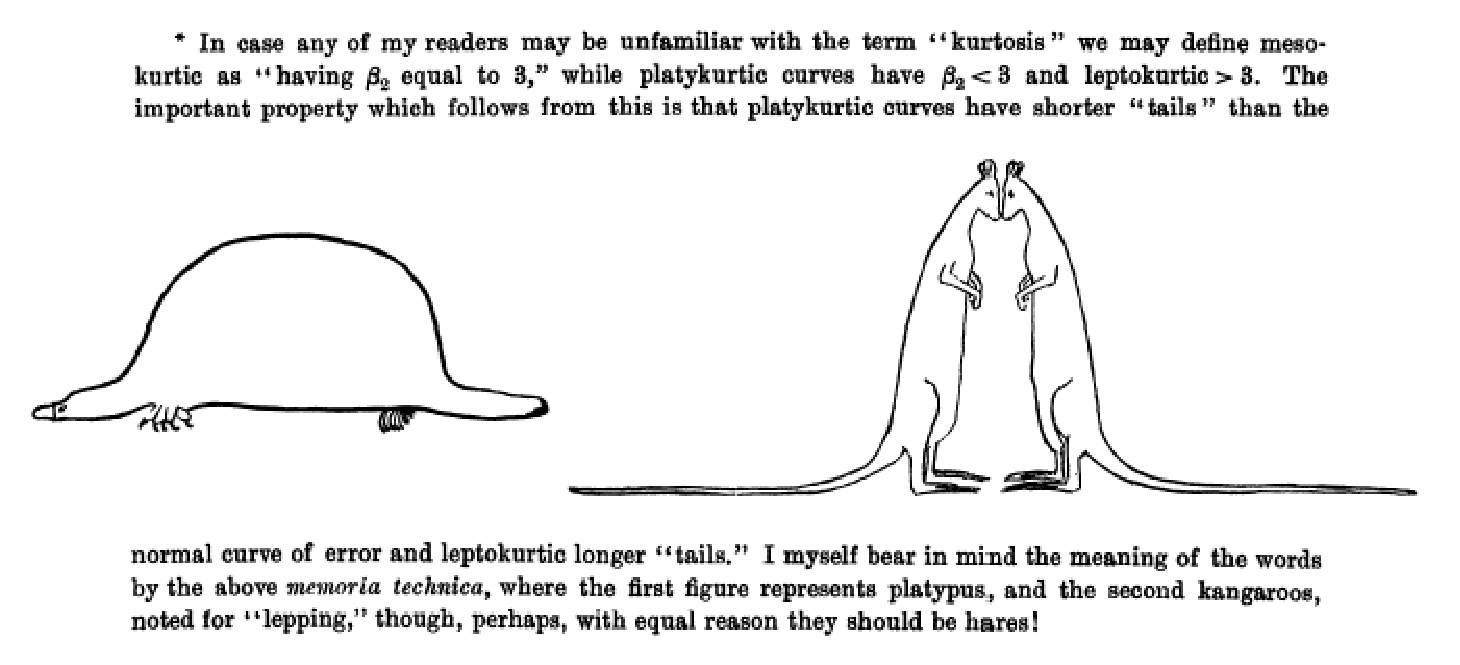
\includegraphics{kurtosis.eps}}
\caption{Leptokurtic, \ind{mesokurtic} and \ind{platykurtic}, illustration by Gosset in {\em Biometrika} \citep[p 160]{student:errors}.\index{Student} \index{William S Gosset}\index{leptokurtic}}
\label{tailfig}
\end{figure*}

We have already written everything we need to calculate all of these easily.
Since the skew and kurtosis are both the mean of an iid process (recall
their definitions on page \pageref{kurtskew}: a sum over $n$), their
square is $\sim \chi^2$. Thus,
$$L_s = n\left[{{\rm skew}^2\over 6}\right]$$
has a $\chi^2$ distribution with one degree of freedom, as does
$$L_k = n\left[{({\rm kurtosis}-3)^2\over 24}\right].$$
Some prefer to test both simultaneously using
$$L_{sk} = n\left[{{\rm skew}^2\over 6} + {({\rm kurtosis}-3)^2\over 24}\right],$$
which has a $\chi^2$ distribution with two degrees of freedom. In code:

\begin{lstlisting}
double  skew    = apop_vector_skew(datavector);
double  kurt    = apop_vector_kurtosis(datavector);
double  statistic = n * (gsl_pow_int(skew,2)/6. + gsl_pow_int(kurt -3,2)/24.)
printf("We reject the null that your data is Normal with probability %g.\n", gsl_cdf_chisq_P(statistic, 2));
\end{lstlisting}

Another alternative, keeping with the theme of this book, would be
to bootstrap the variance of the kurtosis, which would let you find a
confidence interval around $3 \sigma^4$ and state with some percentage
of certainty that the kurtosis is or is not where it should be.
